\documentclass{beamer}

% Gerado a partir de poster.tex.in por preencher_numeros.py: os números entre
% @@...@@ vêm de docs/avaliacao_professor/resultados/resumo.json.

% ====================
% Packages
% ====================

\usepackage[size=custom, width=160,height=90, scale=1.6]{beamerposter}

\usepackage[T1]{fontenc}
\usepackage[utf8]{luainputenc}
\usepackage{lmodern}
\usepackage[sfdefault]{roboto}


\usetheme{gemini}
\usecolortheme{mit}

\usepackage{graphicx}
\usepackage{booktabs}
\usepackage{tikz}
\usepackage{pgfplots}
\pgfplotsset{compat=1.14}

\usepackage{anyfontsize}
\usepackage{fontawesome5}

\usepackage{lipsum}
% citações numéricas: o formato autor-ano do modelo saía quebrado nesta
% instalação ("Fox1972]")
\usepackage[square,numbers]{natbib}
\usepackage{tabularx}
\usepackage{siunitx}
\sisetup{detect-all}
\usepackage{amsfonts}
\usepackage{amsmath}
\usepackage{amssymb}

\hyphenpenalty=10000

\usetikzlibrary{positioning,arrows.meta}
\deftranslation[to=English]{Figure}{Figura}


% ====================
% Lengths
% ====================

% If you have N columns, choose \sepwidth and \colwidth such that
% (N+1)*\sepwidth + N*\colwidth = \paperwidth

\newlength{\sepwidth}
\newlength{\colwidth}

% 2 columns
%\setlength{\sepwidth}{0.025\paperwidth}
%\setlength{\colwidth}{0.4625\paperwidth}
\setlength{\sepwidth}{0.025\paperwidth}
\setlength{\colwidth}{0.3\paperwidth}

\newcommand{\separatorcolumn}{\begin{column}{\sepwidth}\end{column}}

% ====================
% Title
% ====================

\title{Clima Brasil: plataforma web para explorar o clima dos municípios brasileiros e o El Niño}

\author{Filipe Nascimento Soares e Guilherme Marinheiro de Oliveira}

\institute[shortinst]{Bacharelado em ciência da computação, IF Goiano - Campus Rio Verde}

% ====================
% Footer (optional)
% ====================

\footercontent{
    \href{https://github.com/lipe14-ops/projeto-integrador-2}{\faGithub\hspace{0.5ex} lipe14-ops/projeto-integrador-2}
    \hspace{5cm}
    \href{mailto:filipe.soares@estudante.ifgoiano.edu.br}{\faEnvelope\hspace{0.5ex} filipe.soares@estudante.ifgoiano.edu.br}
    \hspace{5cm}
    \href{mailto:guilherme.marinheiro@estudante.ifgoiano.edu.br}{\faEnvelope\hspace{0.5ex} guilherme.marinheiro@estudante.ifgoiano.edu.br}
}
% (can be left out to remove footer)

% ====================
% Logo (optional)
% ====================

% use this to include logos on the left and/or right side of the header:
% Left: institution
\logoright{
\includegraphics[height=7cm]{logos/logo_if.png}}
% Right: funding agencies and other affilations
%\logoright{\includegraphics[height=7cm]{logos/NSF.eps}}
% ====================
% Body
% ====================

\begin{document}
%\large

	\begin{frame}[t]
		\begin{columns}[t]

			%%%%%%%%%%%%% Primeira coluna
			\separatorcolumn
			\begin{column}{\colwidth}
				%%%%%%%%%%%%% Resumo
			    \begin{block}{Resumo}
			    	\small{O Clima Brasil é uma plataforma web gratuita para explorar o clima dos 5.570 municípios
			    	brasileiros de 2015 a 2025, com os períodos de El Niño e La Niña em destaque, comparação entre
			    	municípios, dias de chuva fora do padrão com notícias da época e um mapa nacional.}
			    \end{block}

				%%%%%%%%%%%%% Introdução
			    \begin{block}{Introdução}
			        O El Niño aquece o Pacífico Equatorial e costuma trazer seca ao Norte e ao Nordeste e chuva
			        intensa ao Sul. Os dados climáticos existem, mas estão espalhados e são difíceis de explorar.
			        A plataforma responde a:

			        \begin{enumerate}
			        	\item \textbf{Impacto local:} como foi o clima de um município durante o El Niño e a La Niña?
			        	\item \textbf{Comparação:} como dois municípios se diferenciam?
			        	\item \textbf{Eventos:} quando choveu fora do padrão, e o que os jornais disseram?
			        \end{enumerate}
			    \end{block}

				%%%%%%%%%%%%% Trabalhos relacionados
			    \begin{block}{Trabalhos relacionados}

			        \begin{itemize}
			        	\item \citet{vianna2021estacoes}: em SC há estações suficientes, mas mal distribuídas.
			        	\item \citet{ribeiro2026ml}: processam séries longas do INMET por município.
			        	\item \citet{roth2013interactive}: o mapa interativo é ferramenta de raciocínio.
			        	\item \citet{leigh2019framework}: ARIMA detecta anomalias em rios; base do método adotado.
			        \end{itemize}
			        \textbf{Lacuna:} nenhum liga, de forma visual, o clima de cada município ao El Niño.
			    \end{block}

				\begin{alertblock}{Metodologia}
					\begin{itemize}
						\item \textbf{Dados:} reanálise ERA5-Land~\citep{munozsabater2021era5land} (grade de $\sim$9\,km).
						\item \textbf{IBGE:} malha municipal, código, região, população, bioma, relevo e área.
						\item \textbf{El Niño e La Niña:} índice ONI da NOAA, em faixas atrás dos gráficos.
						\item \textbf{Notícias:} busca matérias de 3 dias antes a 7 depois do evento e confere data,
						cidade e tema na página original~\citep{tarhule2005sahel,yagoub2020newspapers}. Teste com 67
						notícias simuladas e gabarito prévio: 91\% das corretas aceitas, 72\% de acerto (F1 = 0,81).
					\end{itemize}

					\begin{center}
						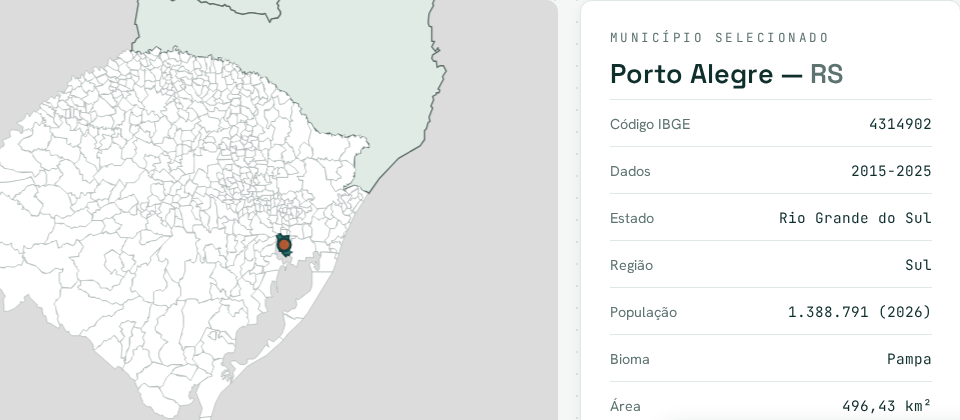
\includegraphics[width=0.26\linewidth]{figures/tela_ibge_recorte.png}\\
						\small Malha municipal e ficha do município com dados do IBGE.
					\end{center}


			    \end{alertblock}
			\end{column}

			%%%%%%%%%%%%% Segunda coluna
			\separatorcolumn
			\begin{column}{\colwidth}
				%%%%%%%%%%%%% Metodologia
				\begin{alertblock}{Metodologia}
					\textbf{Como os dados chegam até o site:}

					\vspace{1ex}
					{\centering
					\begin{tikzpicture}[
						node distance=1.2cm and 1.4cm,
						caixa/.style={draw=mitred, fill=white, rounded corners=6pt, line width=2pt,
							align=center, minimum height=4cm, text width=12.2cm, inner sep=0.4cm},
						seta/.style={-{Latex[length=0.9cm,width=0.8cm]}, line width=3pt, draw=mitred}]
						\node[caixa] (dados) {\faCloudSunRain\\[0.4ex]\textbf{Dados}\\\small ERA5-Land, IBGE
						e NOAA};
						\node[caixa, right=of dados] (banco) {\faDatabase\\[0.4ex]\textbf{Banco}\\\small
						PostgreSQL + PostGIS};
						\node[caixa, right=of banco] (analise) {\faChartLine\\[0.4ex]\textbf{Análise}\\\small dias
						fora do padrão};
						\node[caixa, below=of analise] (noticias) {\faNewspaper\\[0.4ex]\textbf{Notícias}\\\small
						busca e conferência};
						\node[caixa, left=of noticias] (api) {\faServer\\[0.4ex]\textbf{API}\\\small FastAPI};
						\node[caixa, left=of api] (site) {\faGlobeAmericas\\[0.4ex]\textbf{Site}\\\small React +
						Leaflet};
						\draw[seta] (dados) -- (banco);
						\draw[seta] (banco) -- (analise);
						\draw[seta] (analise) -- (noticias);
						\draw[seta] (noticias) -- (api);
						\draw[seta] (api) -- (site);
					\end{tikzpicture}\par}

					\begin{itemize}
						\item \textbf{Navegação:} Brasil $\rightarrow$ estado $\rightarrow$ município, com
						gráficos mensais, comparação entre municípios e download dos dados.
						\item \textbf{Dias fora do padrão:} um modelo estatístico (ARIMA) prevê a chuva de cada
						dia~\citep{hyndman2021fpp,leigh2019framework}. O ``resíduo'' é o erro dessa previsão; se for
						maior que 3 desvios-padrão ($Z>3$), o dia é \emph{anomalia}. Ele só é \emph{extremo} se o
						volume também for \textbf{raro}: maior que o de 95\% dos dias de chuva do município nos anos
						anteriores (percentil 95), por exemplo 33\,mm em Porto Alegre e 21\,mm em Rio Verde. Assim,
						38,1\% das anomalias não são extremas.
					\end{itemize}
				\end{alertblock}

				\begin{exampleblock}{A plataforma}

					\heading{Gráficos com El Niño e La Niña}

					\begin{center}
						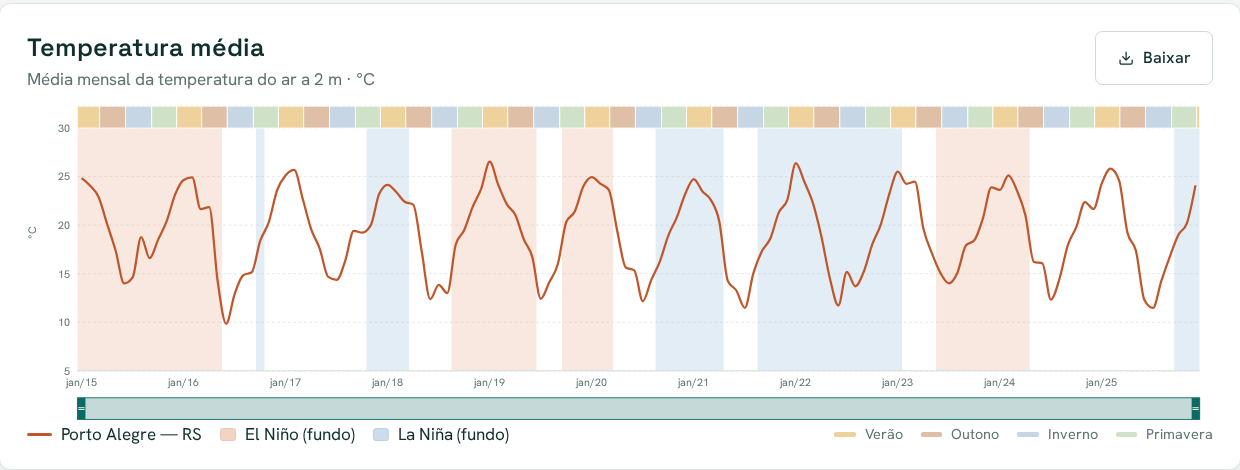
\includegraphics[width=0.32\linewidth]{figures/tela_graficos_recorte.png}
					\end{center}

					\heading{Eventos de chuva com notícias conferidas}

					\begin{center}
						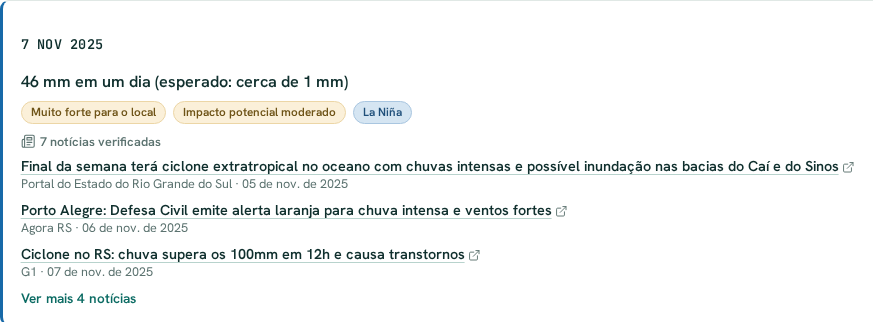
\includegraphics[width=0.46\linewidth]{figures/tela_noticia_evento.png}
					\end{center}

					\small
					\textbf{Cada evento:} data, chuva (dia ou 3--5 dias), classificação para o local, impacto
					potencial, fase do ENSO e notícias. \textbf{Cada notícia:} manchete, veículo, data, link,
					confiabilidade da fonte e se é do município ou de um vizinho. \textbf{Limitação:} o verificador
					ainda aceita previsões e alertas (como os dois primeiros itens) como notícia do evento.
					\normalsize

				\end{exampleblock}
			\end{column}

			%%%%%%%%%%%%% Terceira coluna
			\separatorcolumn
			\begin{column}{\colwidth}

			    %%%%%%%%%%%%% Resultados
			    \begin{block}{Resultados}
			        \begin{figure}
			            \centering
			            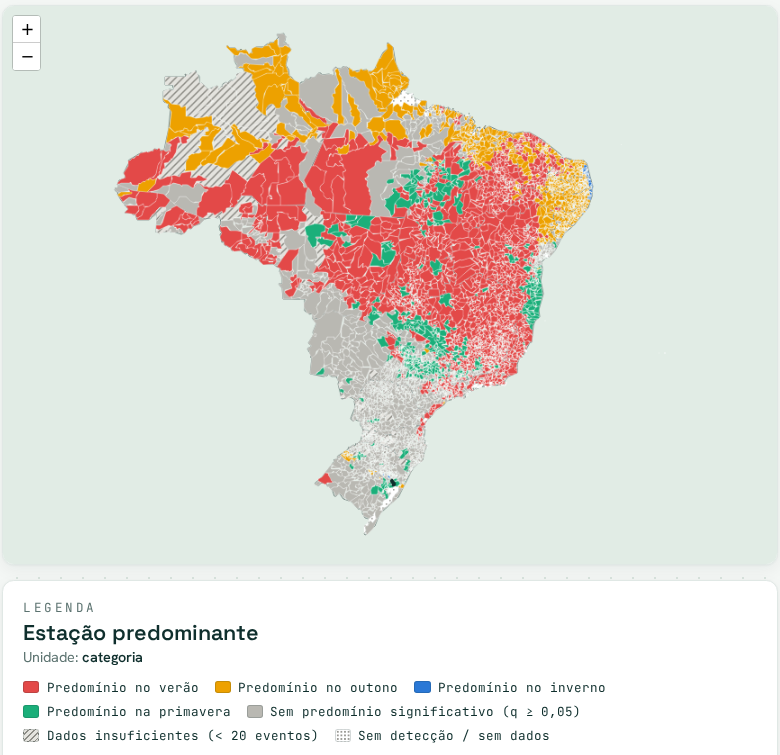
\includegraphics[width=0.25\columnwidth]{figures/tela_mapa_nacional_recorte.png}
			            \caption{Mapa coroplético: estação com mais eventos de chuva por município.}
			            \label{fig:mapa}
			        \end{figure}

			        Respostas obtidas na plataforma (Explorar e Mapa nacional):
			        \begin{enumerate}
			        	\item \textbf{Impacto local:} gráficos de qualquer município com El Niño e La Niña ao fundo
			        	(leitura visual, não causal).
			        	\item \textbf{Comparação:} Porto Alegre teve 54,8\% dos eventos no outono/inverno (50\% =
			        	sem preferência), traço fraco do Sul; no Brasil, o verão predomina em 37,3\% dos municípios
			        	e o inverno em 0,9\% (Figura~\ref{fig:mapa}).
			        	\item \textbf{Eventos:} quanto mais forte a chuva, mais notícias confirmam o evento (18\%
			        	abaixo de 20\,mm; 37\% nos acumulados extremos).
			        \end{enumerate}
			    \end{block}

				%%%%%%%%%%%%% Conclusão
			    \begin{block}{Conclusão}
			    	Contra a dispersão dos dados, o site reúne 46,6 milhões de registros de 5.535 municípios e
			    	responde às três perguntas com um método validado~\citep{leigh2019framework}.
			    	\textbf{Próximos passos:} comparar com o INMET e avaliar as notícias por humanos.
			    \end{block}

			    \begin{block}{Referências}
				%	    \nocite{*}
					\scriptsize{\bibliographystyle{unsrtnat}\bibliography{references}}
			    \end{block}

			\end{column}

			\separatorcolumn
		\end{columns}

	\end{frame}

\end{document}
